\documentclass{standalone}
%
\usepackage{tikz}
\usetikzlibrary{backgrounds,shapes.callouts}
\usepackage{tkz-euclide}
\usepackage{xcolor}
\usepackage{ifthen}
%
\definecolor{space}{HTML}{1F2C4E}
\definecolor{earth}{HTML}{0089FA}
\definecolor{mercury}{HTML}{846549}
\definecolor{venus}{HTML}{BB9765}
\definecolor{mars}{HTML}{DC7B4E}
\definecolor{dida}{HTML}{FFDE00}
\definecolor{title}{HTML}{FBA706}
\definecolor{moon}{HTML}{AFAFAF}
%
\usepackage{fontspec}
\setmainfont{Open Dyslexic}
%
\title{I primi modelli del Sistema Solare}
\begin{document}
	\tikzset{
		partial ellipse/.style args = {#1:#2:#3}{insert path={+ (#1:#3) arc (#1:#2:#3)}},
		notice/.style  = { draw, ellipse callout, callout relative pointer={#1} },
	}
	\begin{tikzpicture}[background rectangle/.style={fill=white},show background rectangle,>={[inset=0,angle'=27]Stealth}]
		%
		\edef\rsun{2}
		\def\fact{8}
		%
		\def\uam{\fact*0.387}
		\def\rmer{0.2}
		%
		\def\uav{\fact*0.723}
		\def\rven{0.5}
		%
		\def\uaet{\fact*1}
		\def\ret{0.53}
		%
		\def\uams{\fact*1.52}
		\def\rms{0.28}
		%
		%title
		\draw [black,ultra thick,fill=title] (0,9.8) rectangle (30,16.8);
		\node at (15,14.8) {\textcolor{black}{\fontsize{80}{81}\selectfont I primi modelli}};
		\node at (15,11.8) {\textcolor{black}{\fontsize{80}{81}\selectfont del Sistema Solare}};
		%
		\begin{scope}[shift={(0,5)}]
			\node at (23,0) {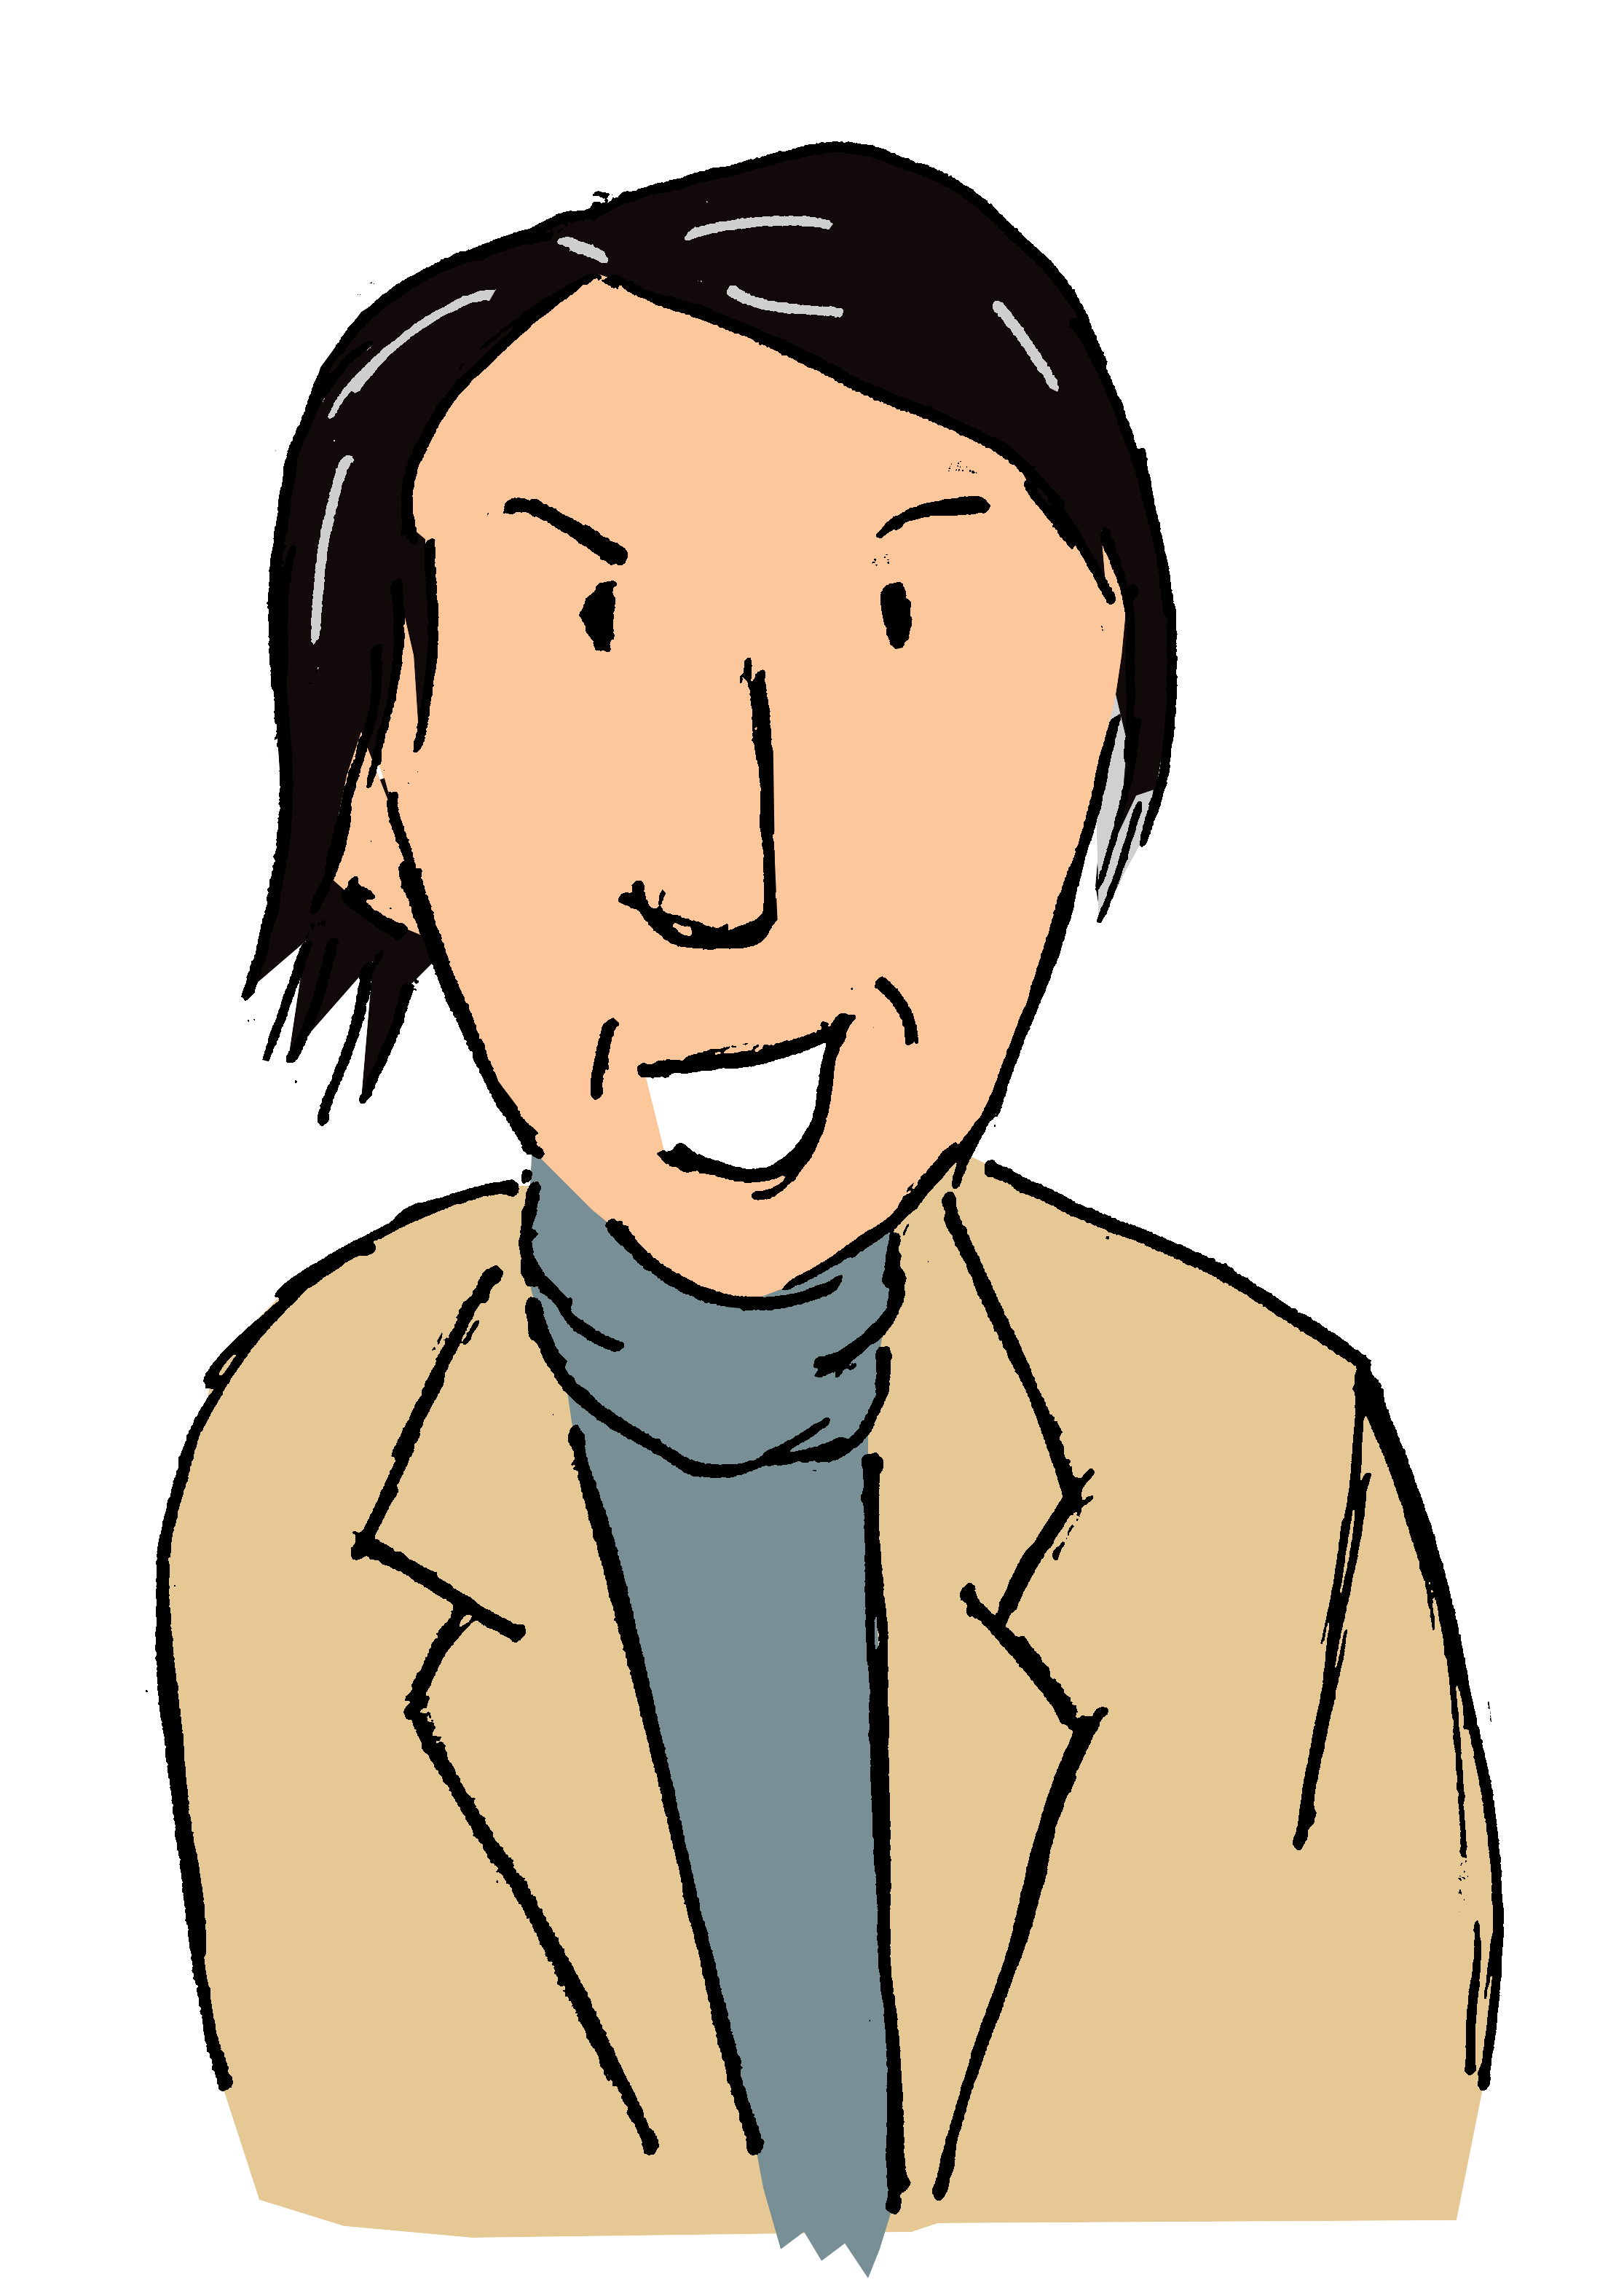
\includegraphics[width=5cm]{img/carl_sagan}};
			\node (example-textwidth-2) [notice={(3,0.5)}, ultra thick, right, align=center, text width=12cm, color=black, fill=white, font=\fontsize{23pt}{24pt}\selectfont] at (1,-1) {Piu' che modelli del Sistema Solare, si dovrebbe parlare di visioni dell'universo. La versione dei miti greci era abbastanza \emph{naif}: una Terra piatta circondata dall'oceano, un fiume, con il Tartaro sotto di essa:};
		\end{scope}
		%
		\begin{scope}[shift={(0,-9)}]
			\node at (15,0) {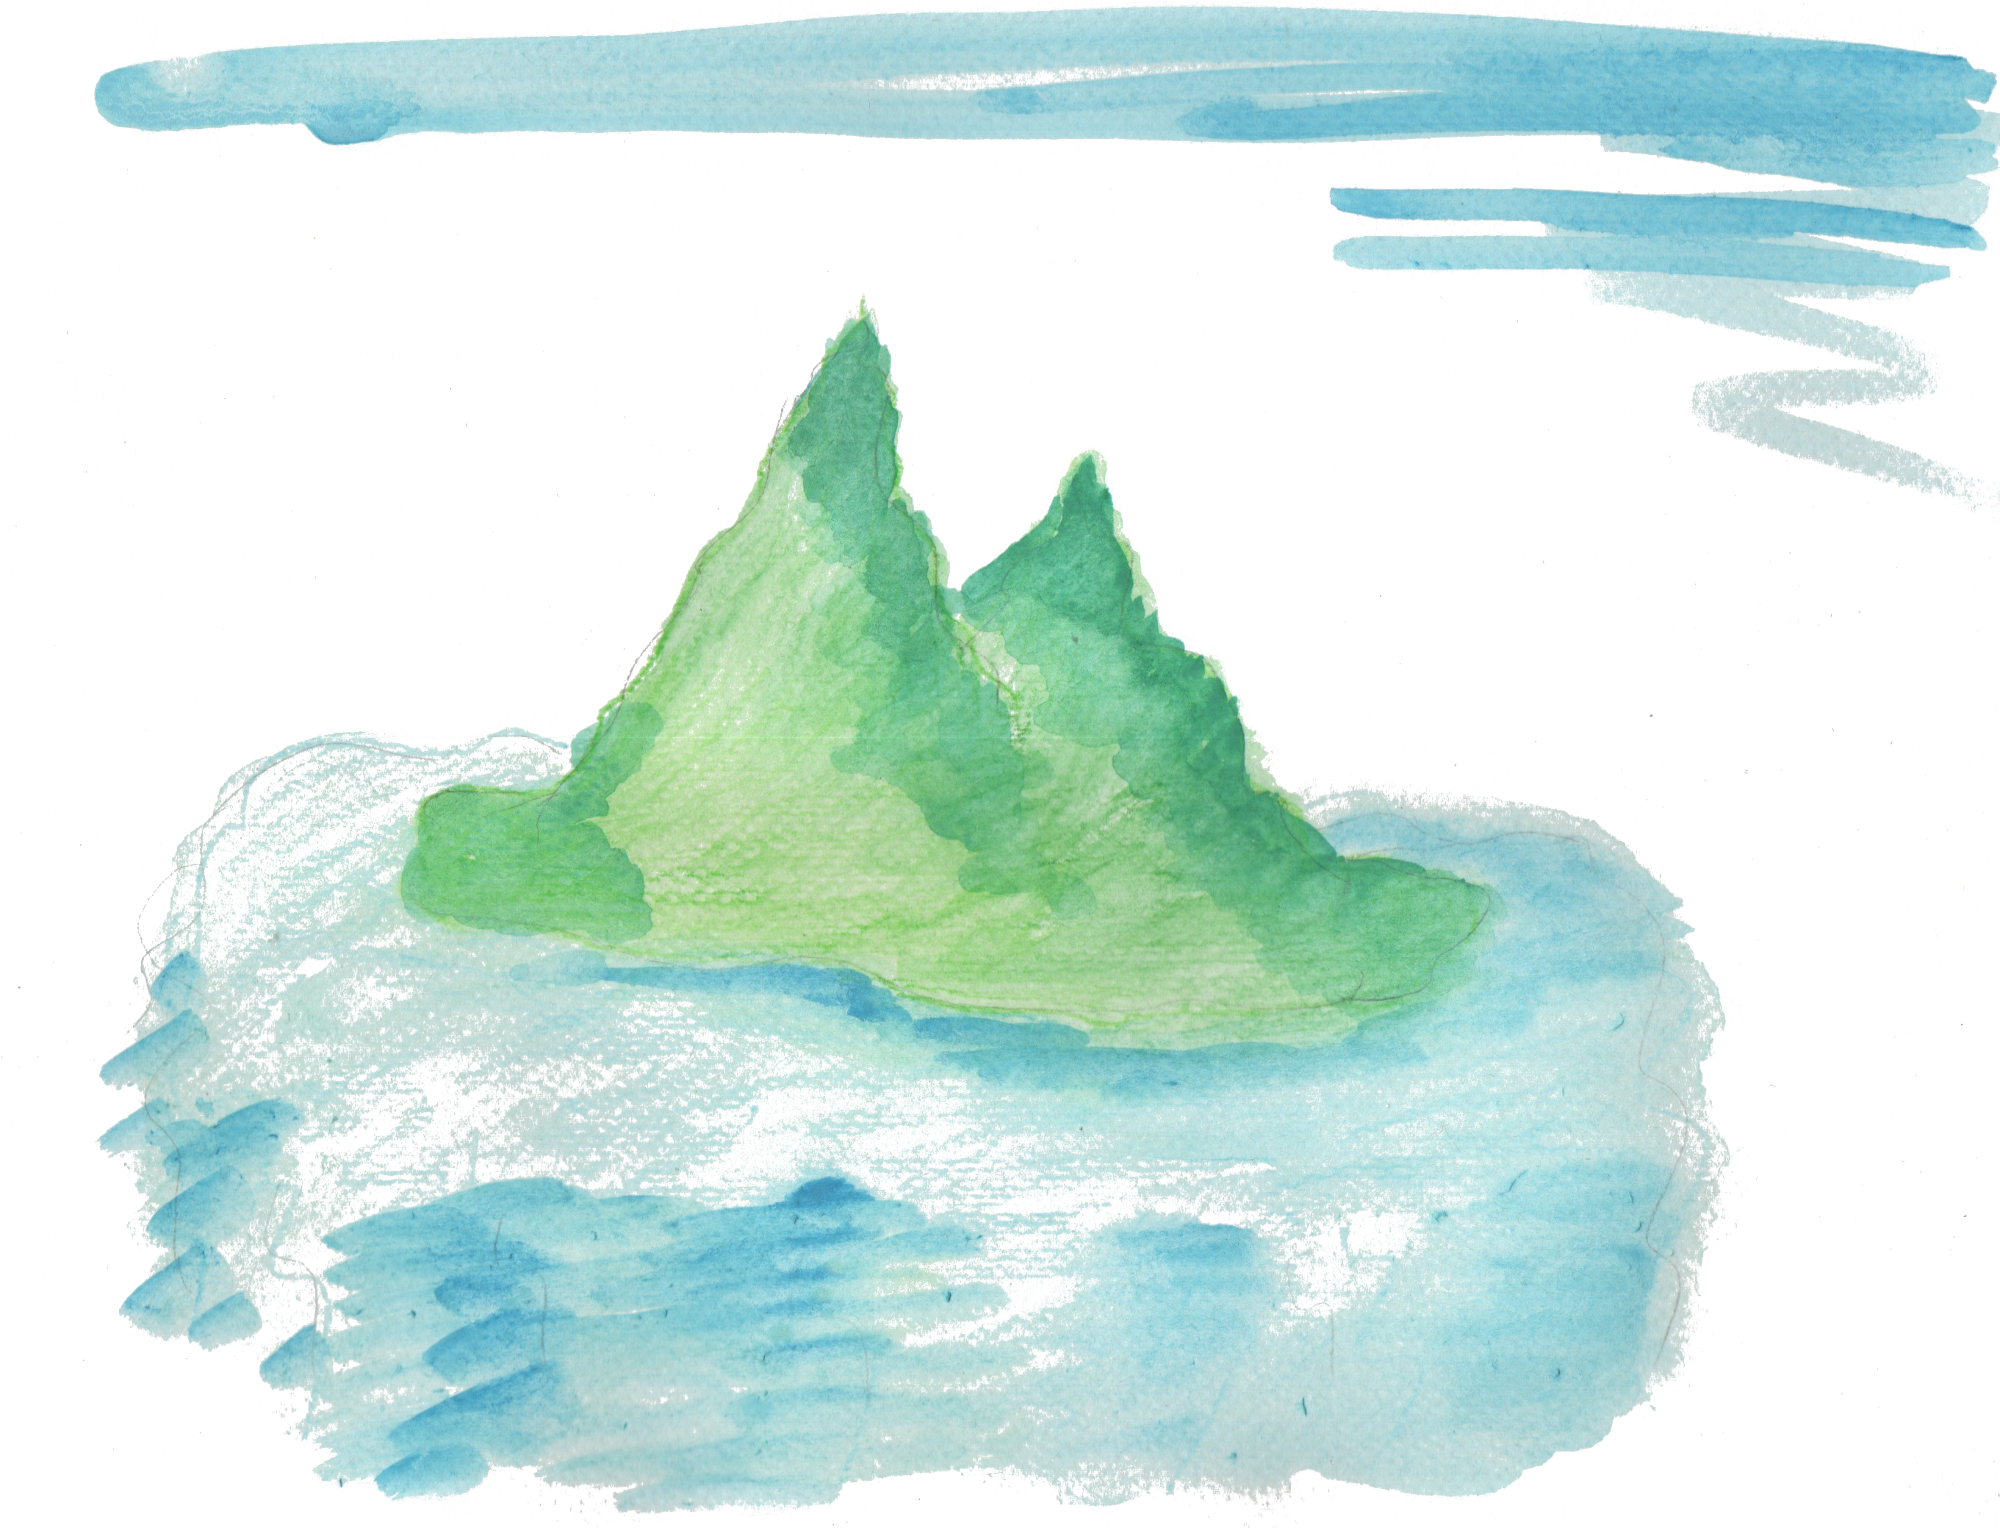
\includegraphics[width=20cm]{img/island}};
			\node at (8,5) {
\includegraphics[width=3cm]{img/carro_sole}};
		\end{scope}
		%
		\begin{scope}[shift={(0,-19)}]
			%
			\draw [fill=dida, ultra thick] (1,2) rectangle (27.5,-2);
			\node (example-textwidth-2) [right, align=left, text width=26cm, color=black, font=\fontsize{23pt}{24pt}\selectfont] at (1.5,0) {A rimuovere questa visione ci penso' Parmenide, che scopri' la sfericita' della Terra e la prima spiegazione delle fasi lunari.};
			%
		\end{scope}
		%
		\begin{scope}[shift={(0,-26)}]
			\node at (23,0) {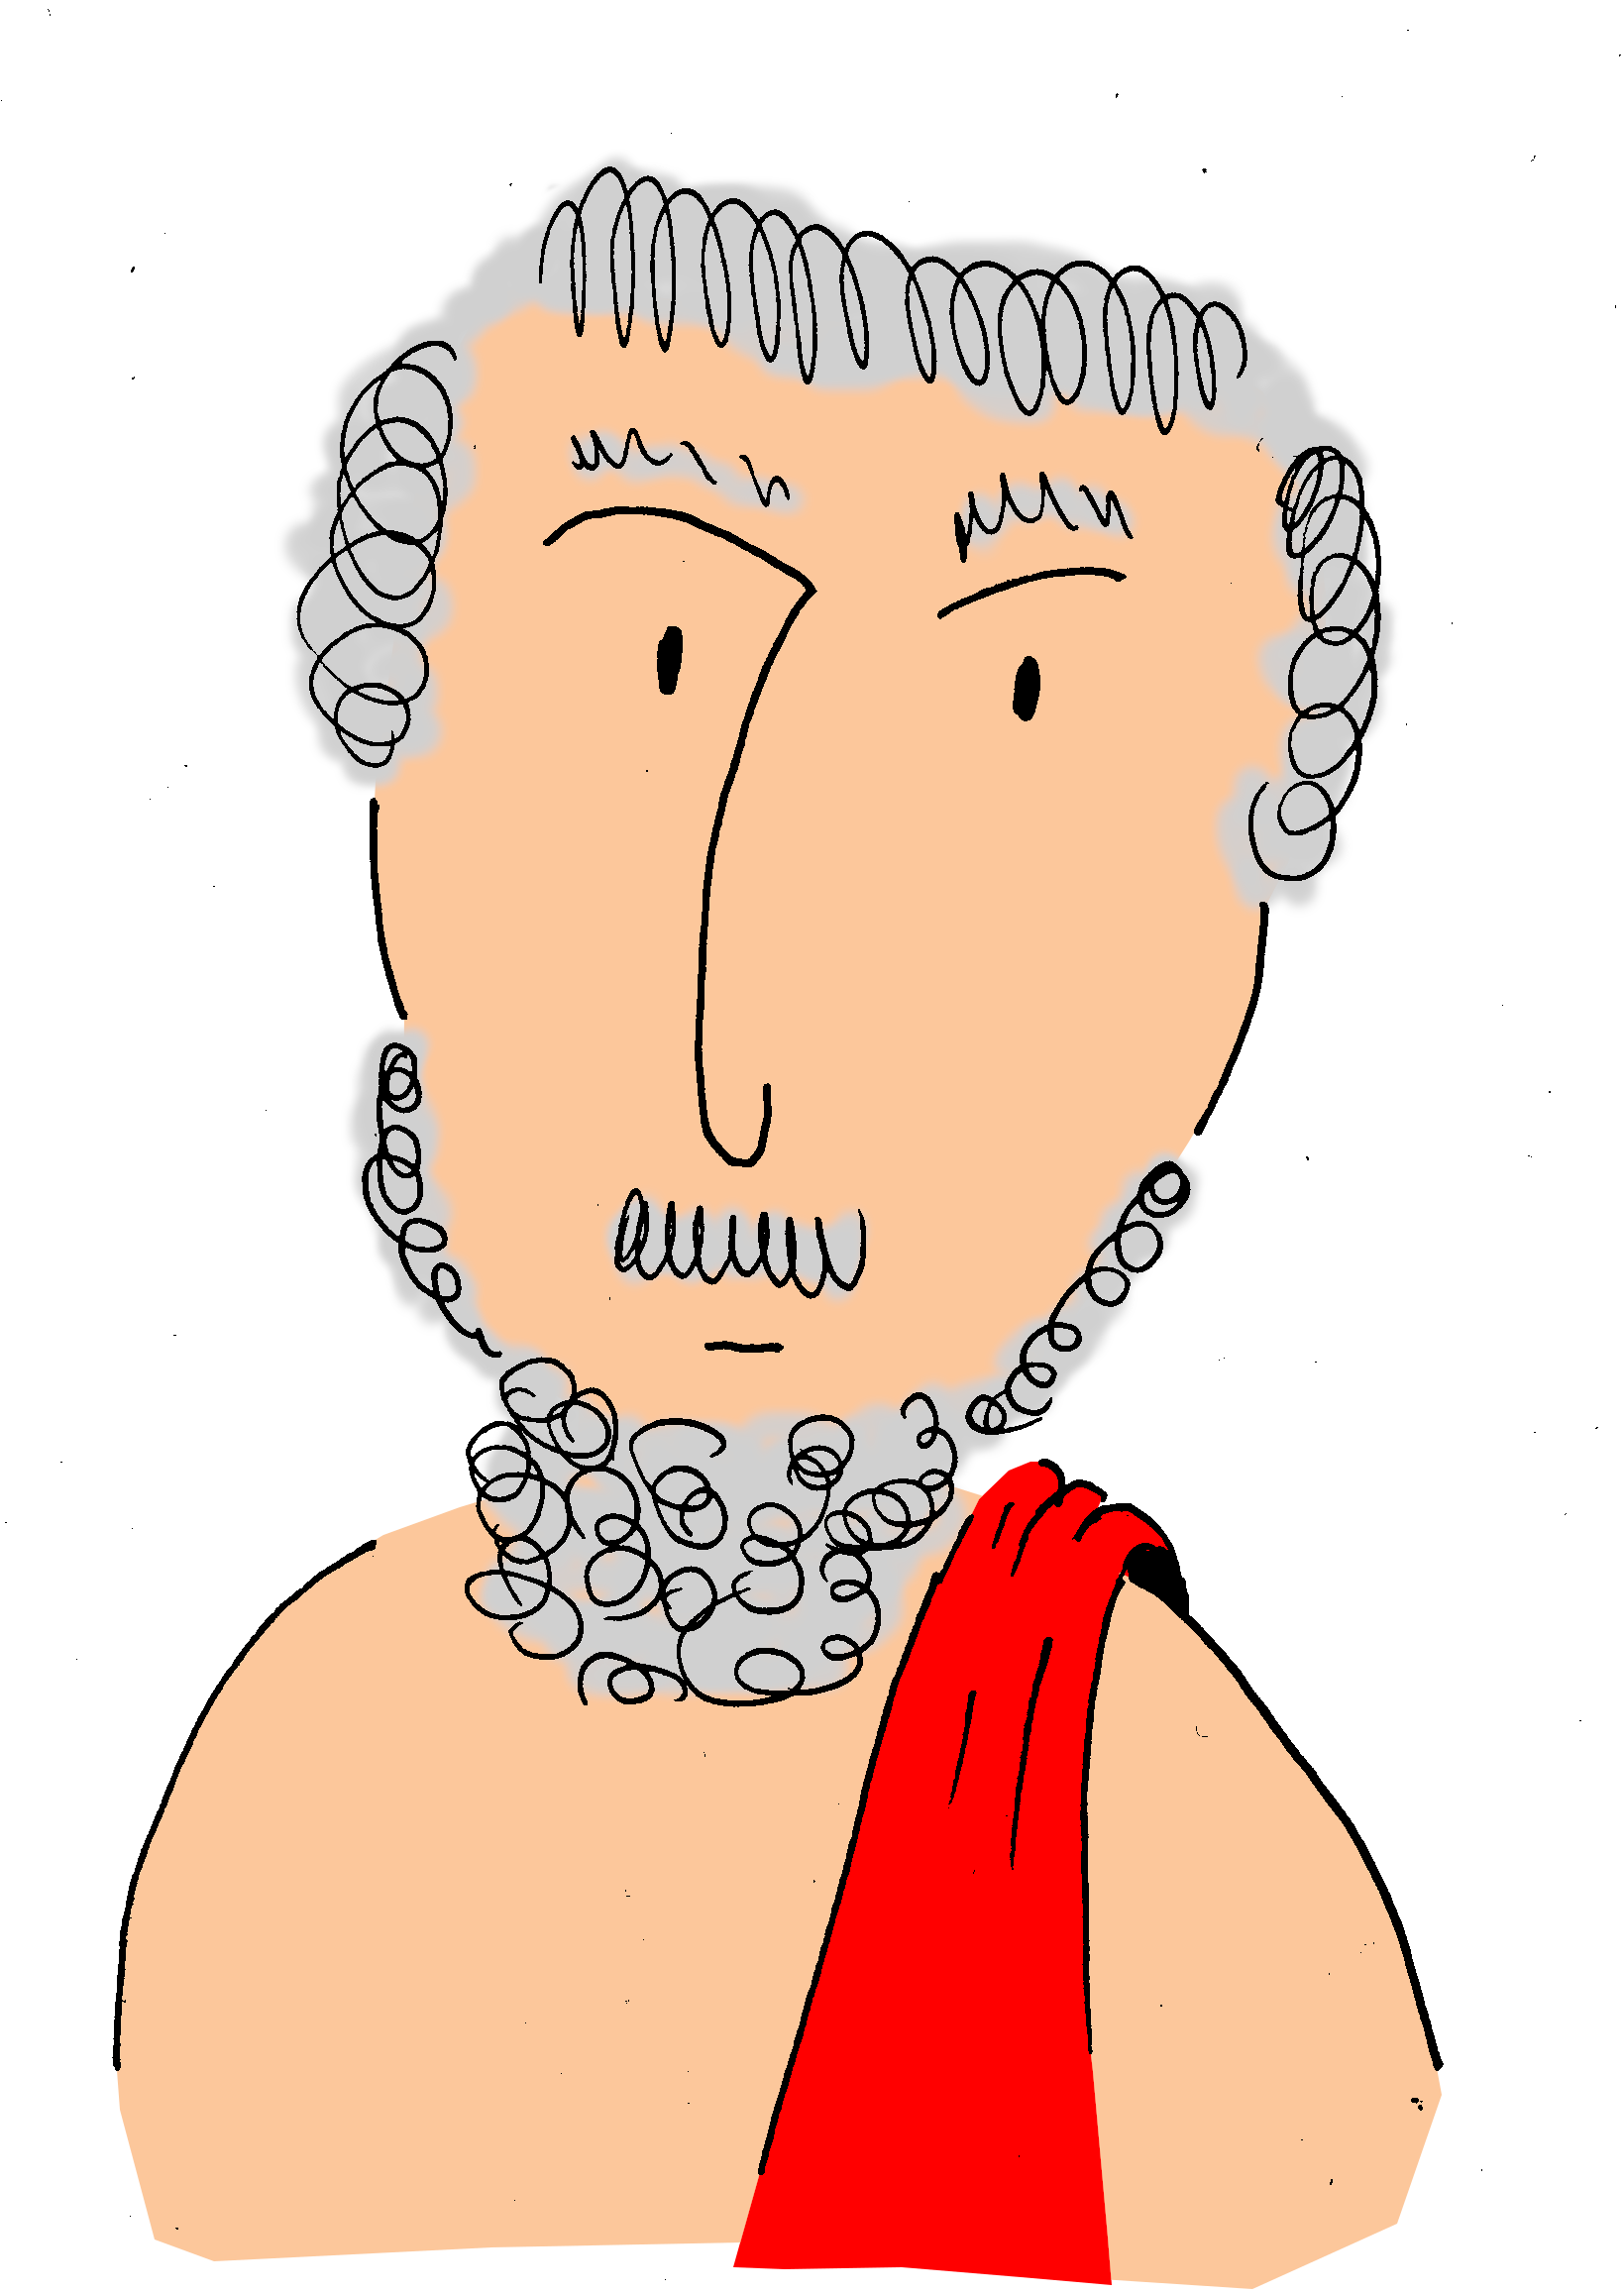
\includegraphics[width=8cm]{img/parmenide}};
			\node (example-textwidth-2) [notice={(3,0.5)}, ultra thick, right, align=center, text width=10cm, color=black, fill=white, font=\fontsize{22pt}{23pt}\selectfont] at (1,-1) {Nel frattempo il mio collega filosofo, il pitagorico Iceta di Siracusa, fu il primo a sostenere la rotazione della Terra su se stessa come spiegazione della rotazione apparente della volta celeste.};
		\end{scope}
		%
		\begin{scope}[shift={(0,-34)}]
			%
			\draw [fill=dida, ultra thick] (1,1.5) rectangle (27.5,-1.5);
			\node (example-textwidth-2) [right, align=left, text width=26cm, color=black, font=\fontsize{23pt}{24pt}\selectfont] at (1.5,0) {Il primo modello vero e proprio venne proposto dal pitagorico Filolao:};
			%
		\end{scope}
		%
		\begin{scope}[shift={(15,-52)},rotate around={-90:(0,0)}]
			\tkzDefPoint(0,0){S1}
			%
			\tkzDefShiftPoint[S1](0:\rsun+\uam){E1}
			\tkzDefShiftPoint[E1](0:\ret){e1}
			\tkzDrawCircle[ultra thick,color=mercury,dashed](S1,E1)
			\tkzDrawCircle[color=black,fill=mercury,ultra thick](E1,e1)
			%
			\tkzDefShiftPoint[S1](0:\rsun+\uav){E2}
			\tkzDefShiftPoint[E2](0:\ret){e2}
			\tkzDrawCircle[ultra thick,color=earth,dashed](S1,E2)
			\tkzDrawCircle[color=black,fill=earth,ultra thick](E2,e2)
			%
			\tkzDefShiftPoint[S1](0:\rsun+\uaet){M1}
			\tkzDefShiftPoint[M1](0:\rmer){m1}
			\tkzDrawCircle[ultra thick,color=moon,dashed](S1,M1)
			\tkzDrawCircle[color=black,fill=earth,ultra thick](M1,m1)
			%
			\tkzDefShiftPoint[S1](0:\rsun+\uams+\rms){M2}
			\tkzDefShiftPoint[M2](0:\rms){m2}
			\tkzDrawCircle[ultra thick,color=mars,dashed](S1,M2)
			\tkzDrawCircle[color=black,fill=mars,ultra thick](M2,m2)
			%
		\end{scope}
		% 
		\begin{scope}[shift={(0,-51)}]
			\node at (15,0) {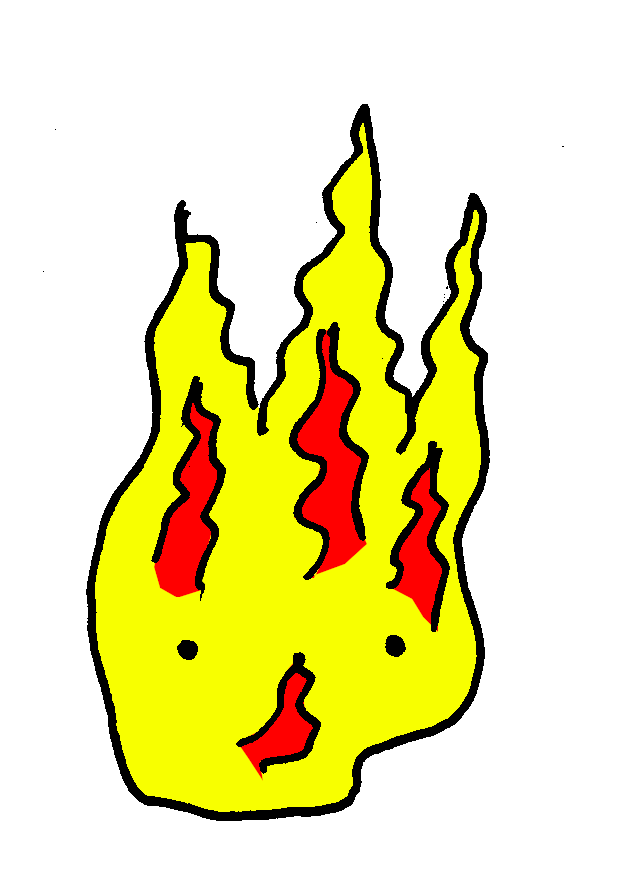
\includegraphics[width=4cm]{img/hestia}};
		\end{scope}
		%
		\begin{scope}[shift={(0,-72)}]
			 \node at (23,0) {
\includegraphics[width=8cm]{img/filolao}};
			 \node (example-textwidth-2) [notice={(3,0.5)}, ultra thick, right, align=center, text width=12cm, color=black, fill=white, font=\fontsize{23pt}{24pt}\selectfont] at (1,-1) {Al centro c'e' Hestia, un fuoco primordiale che riscalda l'universo, mentre intorno a esso ruota l'Anti-Terra, un pianeta oscuro che ci impedisce di vedere Hestia.};
		\end{scope}
		%
		\begin{scope}[shift={(0,-82)}]
			\draw [ultra thick, fill=space] (2.5,1.5) rectangle (28,-2.5);
			\node (example-textwidth-2) [right, align=left, text width=16cm, color=white, font=\fontsize{18pt}{19pt}\selectfont] at (3,-0.5) {Il primo vero modello eliocentrico venne proposto da Aristarco da Samo: la Terra e tutti i pianeti percorrono delle orbite circolari intorno al Sole, mentre le stelle "fisse" appaiono tali a causa della loro enorme distanza da noi.};
			\node at (23,0) {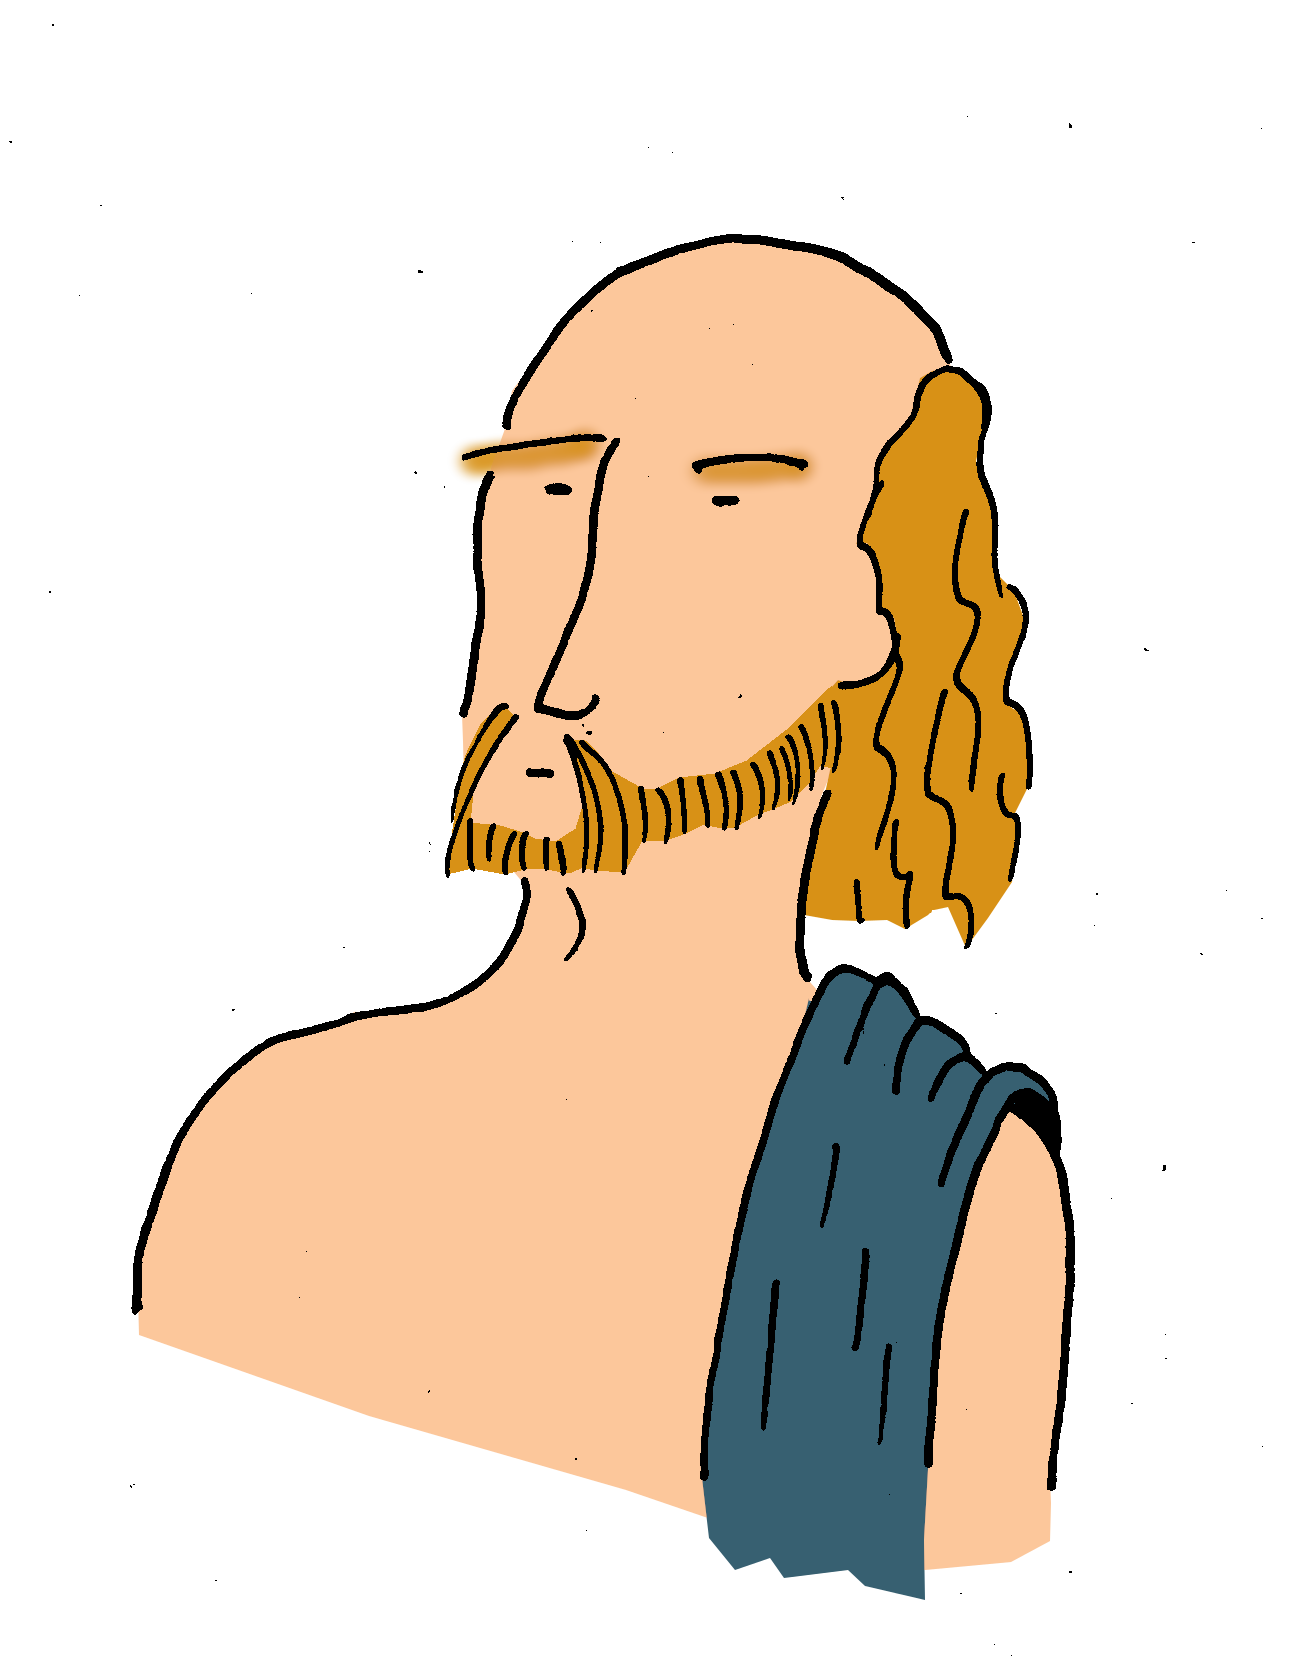
\includegraphics[width=8cm]{img/aristarco}};
		\end{scope}
		%
		\begin{scope}[shift={(0,-90)}]
			\node at (27,0) () {
\includegraphics[width=3.7cm]{img/licenza}};
			\node at (18,-0.1) {\textcolor{black}{\fontsize{14}{15}\selectfont Testo e illustrazioni: @ulaulaman - Gianluigi Filippelli}};
		\end{scope}
	\end{tikzpicture}
%
\end{document}
